\chapter{Gegenüberstellung}

Anhand der unter \ref{qualitätsmetriken} erstellten Metriken sind die Frameworks GeoMesa, Postgres-XL und Rasdaman zu vergleichen.
Der Vergleich findet im Rahmen einer Nutzwertanalyse statt.
Hierbei werden keine Daten von durchgeführten Tests herangezogen, sondern es wird anhand der Spezifikation der einzelnen Frameworks untersucht.\\
%
Die drei Frameworks wurden aus der Tabelle der Abbildung \ref{fig:spatialdatabases} ausgewählt.
\begin{figure}
\centering
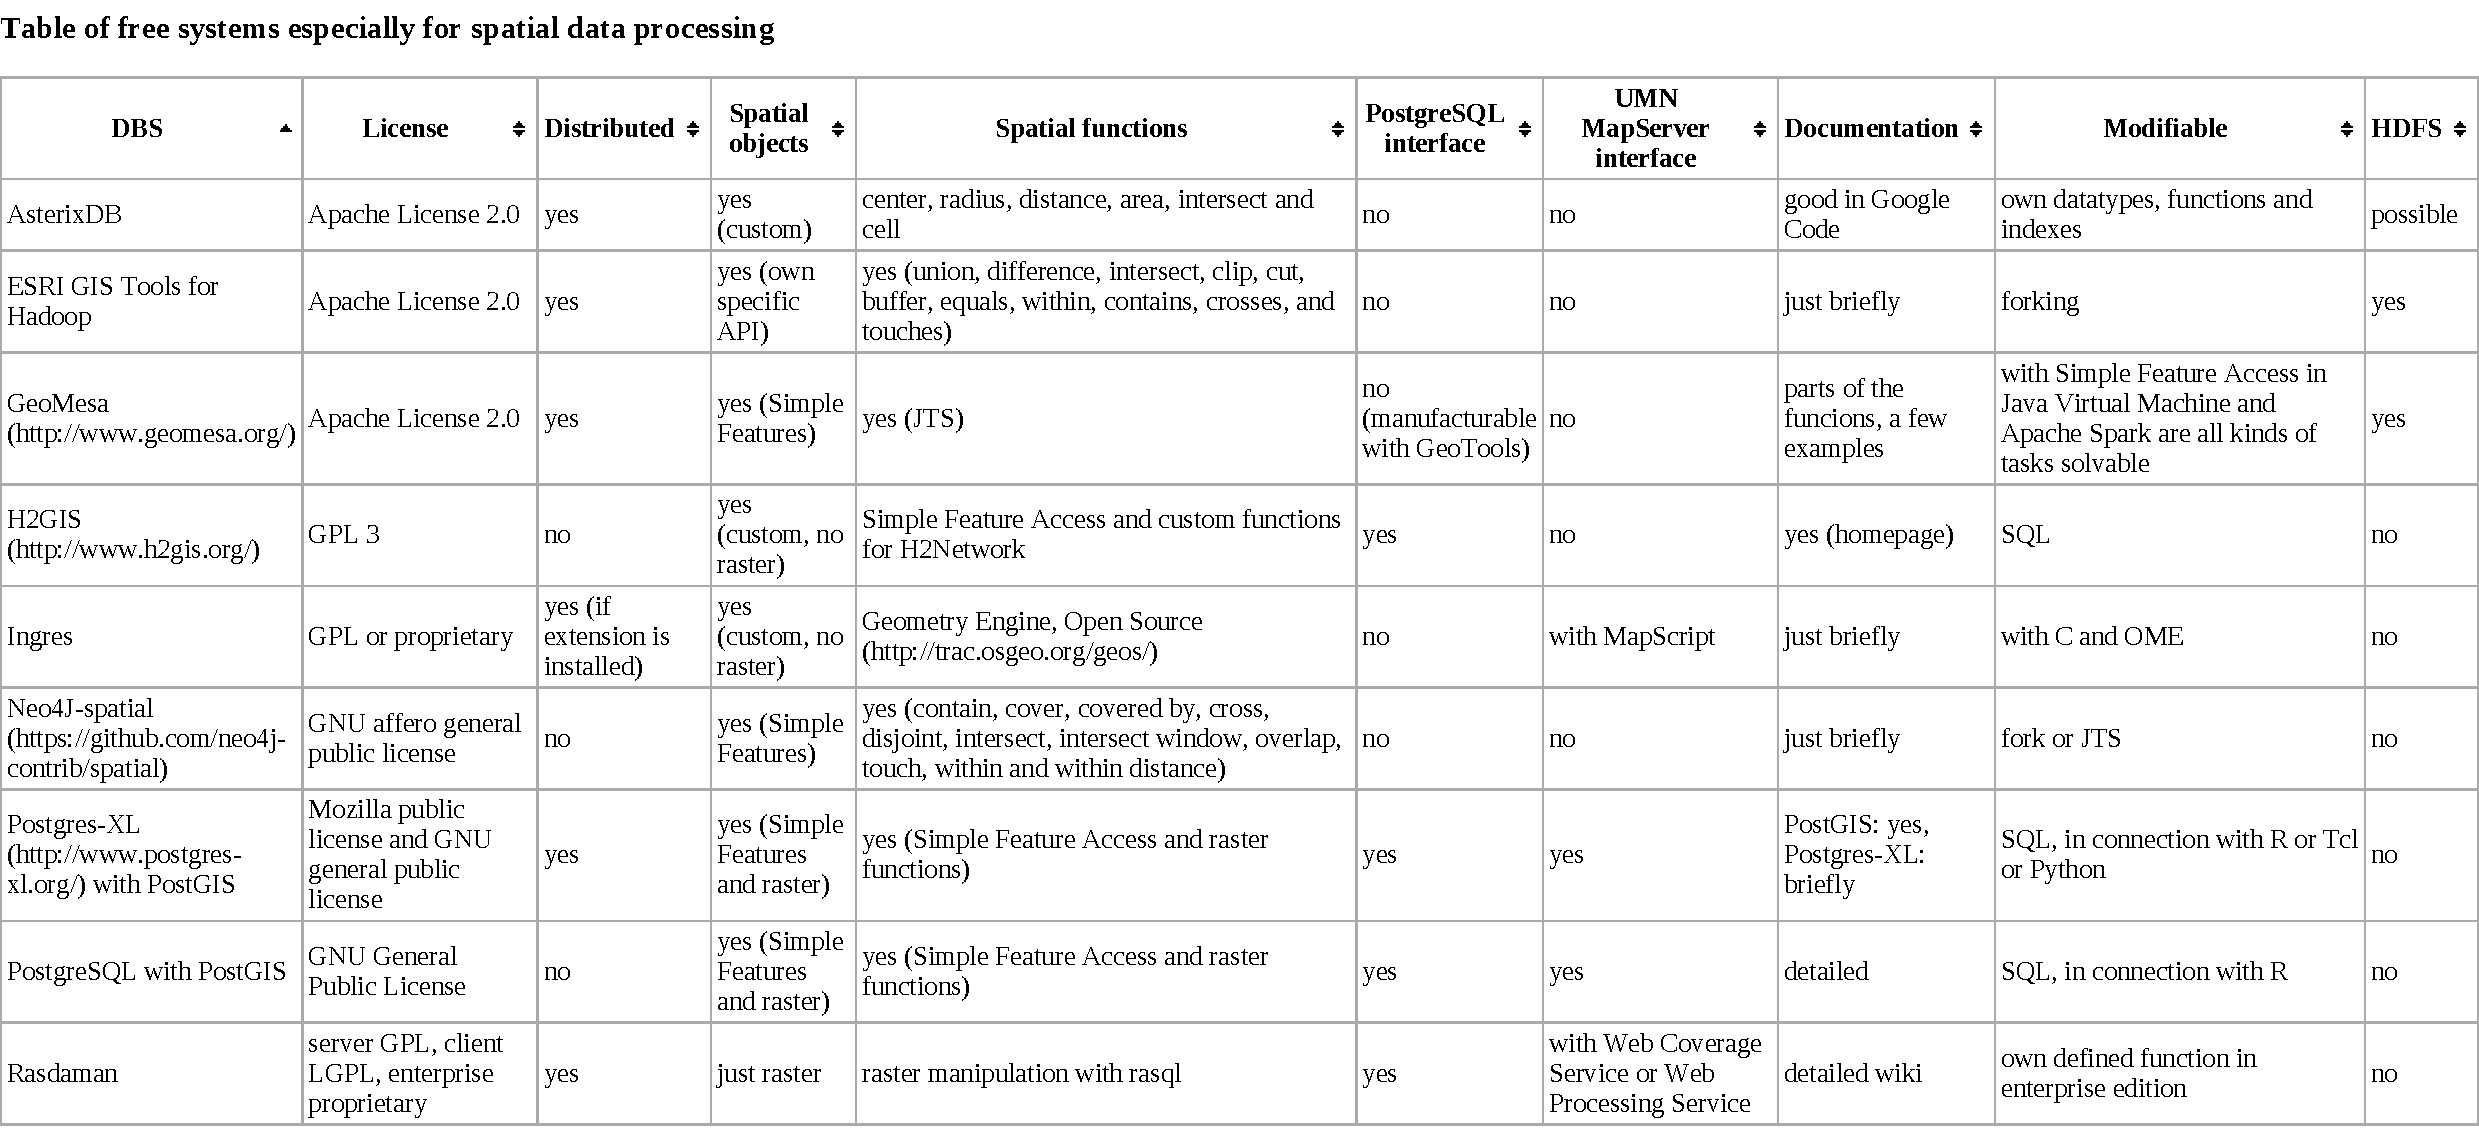
\includegraphics[width=\textwidth]{Abbildungen/table_spatialdatabases_13_2_15.pdf}
\caption[Übersicht relevanter GIS Frameworks]{Übersicht relevanter GIS Frameworks nach \cite{website:wiki-spatialdatabase} vom 2.2.2015}
\label{fig:spatialdatabases}
\end{figure}
Darin sind GIS zur räumlichen Datenverarbeitung mit wesentlichen Eigenschaften wie PostgreSQL Schnittstelle und räumliche Datentypen aufgelistet.
Entsprechend den Anforderungen wurden daraus drei Frameworks für die Nutzwertanalyse ausgewählt.\\
Abbildung \ref{fig:spatialdatabases} stammt von der Wikipedia Seite \url{https://en.wikipedia.org/wiki/Spatial_database} und ist wie unter \ref{aufrufe-spatialdatabases} beschrieben für Unternehmen interessant.
Der Autor erschuf die abgebildete Tabelle durch Recherche und stellte sie am 1.2.2015 in den Artikel.
In der Annahme, dass unternehmensbezogene Besucher der Seite fehlendes ergänzen oder falsches korrigieren würden, dient diese zur Auswahl geeigneter Frameworks.

%TODO: Nutzertanalyse: Struktur, Bewertungssystem, erklären

Tabelle \ref{table:Wertungsmassstab} zeigt die für die Nutzwertanalyse notwendige Wertung der einzelnen Metriken.
\begin{table}[h]
\centering
\begin{tabular}{l|l}
\textbf{Metrik} & \textbf{Gewichtung in \%} \\ \hline
%Richtigkeit & 10 \\ \hline
Interoperabilität & 30 \\ \hline
Funktionsumfang & 20 \\ \hline
%Fehlertoleranz & 8 \\ \hline
Dokumentation & 35 \\ \hline
%Zeitverhalten & 16 \\ \hline
Modifizierbarkeit & 15
\end{tabular}
\caption{Wertungsmaßstab der einzelnen Metriken}
\label{table:Wertungsmassstab}
\end{table}
Die Metriken Richtigkeit, Fehlertoleranz und Zeitverhalten werden nicht in die Analyse aufgenommen, da sie über die Spezifikation nicht belegbar sind.

Für jedes Framework wird eine Nutzwertanalyse durchgeführt und die dazugehörigen Tabellen dazu präsentiert.

Zu jeder Metrik wird der erreichte Wert, die ungewichtete Erfüllung, die gewichtete Erfüllung ein ein Kommentar angegeben.
Die ungewichtete Erfüllung bezieht sich auf den maximal zu erreichenden Wert der Metrik, die gewichtete Erfüllung dagegen auf die Erfüllung der Metrik in Bezug auf \ref{table:Wertungsmassstab}.
Die Kommentarspalte dient der Darstellung des Erreichens der Mindestanforderungen.
Der schlussendliche Nutzwert ergibt sich nach Zangemeister in \cite{website:nutzwertanalyse} aus der Summe der Produkte des Teilnutzens des jeweiligen Kriteriums mit der Gewichtung des Kriteriums.
Der Teilnutzen ist hier der Prozentuale Anteil der erreichten Punktzahl an der maximalen Punktzahl des Kriteriums.
Diese Prozentangabe wird als Wert mit der Gewichtung des Kriteriums multipliziert, woraus sich der Nutzwert für das Kriterium ergibt.
Die Summe aller dieser Teilnutzwerte ergibt den Nutzwert des Frameworks für den Anwendungsfall.

\section{GeoMesa}

\subsection{Interoperabilität}
\begin{description}
\item[PostgreSQL - 7] Scala  kann mit JDBC auf PostgreSQL zugreifen.
\item[\Gls{umn} - 0] \Gls{umn} bietet Accumulo nicht als Quelle an und GeoMesa keine \Gls{ogc} konformen Dienste wie WMS.
\end{description}
Die Wertung für Interoperabilität ist somit 7 mit einer Erfüllung von 58\%.

\subsection{Funktionsumfang}
\begin{description}
\item[Parallele Verarbeitung - 2] Verteilte Datenhaltung durch Accumulo auf \Gls{hdfs} und verteiltes sowie paralleles Rechnen mit beispielsweise Spark \cite{website:geomesaeclipse}
\item[Geografische Datentypen - 12] Vollständige Datentypen aus Simple Feature Access. \cite{website:geomesaeclipse}
\item[Umrechnungsfunktionen - 10] Datenverarbeitung direkt in Spark mit GeoTools möglich. \cite{website:geotools-crs}
\item[Gruppierungsfunktionen - 7] Funktionale Verarbeitung mit Scala.
\item[Verschneidungsfunktionen - 3] \Gls{jts} stellt difference, union und symmetric difference zur Verfügung. \cite{website:jts-wikipedia}
\item[Overlayfunktionen - 2] \Gls{jts} stellt relate und overlay zur Verfügung.
\item[Geostatistik - 0] Keine eingebaute Funktionalität.
\item[Filterfunktionen - 10] Räumliche Filterung ist  mit GeoTools möglich \cite{website:geotools-wiki}
\item[Schemaversionierung - 0] Accumulo erlaubt entsprechend des BigTable Ansatzes ein dynamisches Datenbankschema, jedoch ohne Versionierung. Einzig erzeugte Datentypen, bestehend aus Simple Features, können in GeoMesa als Konstrukt persistiert werden.
\end{description}
Daraus ergibt sich ein Wert von 48, was 79\% des maximal zu erreichenden Wertes ist.

\subsection{Dokumentation}
\begin{description}
\item[Installation - 1] Knappe Hinweise für GeoMesa auf \cite{website:geomesa-quickstart}, dagegen ausführliche Anleitungen für Accumulo auf \cite{website:accumulo-manual}.
\item[Zeitverhalten - 0] Keine Dokumentation vorhanden. %eventuell auf Postgis versus GeoMesa hinweisen
\item[Funktionsumfang - 1] Konkrete Funktionalität von GeoMesa nur grob auf \cite{website:geomesa-tutorials} angedeutet. MapReduce mit Accumulo ist ausführlich beschrieben. \cite{website:accumulo-manual}
\item[Interoperabilität - 1] Nicht explizit bei GeoMesa angegeben, aber Anbindungsmöglichkeiten mit Scala bzw. Java sind im allgemeinen ausführlich dokumentiert.
\item[Best Practise - 0] Keine Dokumentation vorhanden.
\item[Anpassbarkeit - 1] In \cite{website:geomesa-tutorials} sind einige Anregungen zu finden. Beispielsweise die Erzeugung eigener Schemabestandteile. \cite{website:geomesa-simplefeatures}
\end{description}
Das Qualitätskriterium Dokumentation wird für GeoMesa mit dem Wert 4, bzw. der Erfüllung von 31\%,  belegt.

\subsection{Modifizierbarkeit}
\begin{description}
\item[Verwendung eigener Datentypen - 0] Es sind eigene Schemas aber keine Datentypen erstellbar. \cite{website:geomesa-simplefeatures}
\item[Erstellung eigener Schnittstellen - 1] Indirekt über JDBC und ODBC möglich.
\item[Erstellung eigener Funktionen - 1] Durch verschiedenste Frameworks zur Datenverarbeitung wie Spark beliebige Funktionen erstellbar.
\item[Verwendung der Programmiersprachen Scala oder R - 1] GeoMesa ist in Scala geschrieben und kann mit dieser verwendet werden. R kann über das Tool SparkR verwendet werden.
\item[Anlegen eigener Berechnungsvorgängen zur späteren Abarbeitung - 1] Mit einer Vielzahl von Tools möglich, bspw. Spark, \Gls{storm}, Pig und \Gls{cascading}.
\end{description}
Hier ist die Wertung 4 von 5 Punkten und damit 80\%.

\subsection{Zusammenfassung}
\begin{table}[h!]
\centering
\small
\begin{tabular}{l|p{1.8cm}|c|p{3.1cm}|p{1.8cm}}
\textbf{Metrik} & \textbf{erreichter Wert} & \textbf{Erfüllung in \%} & \textbf{Kommentar} & \textbf{gewichteter Teilnutzen} \\ \hline
Interoperabilität & 7 & 58 & Implementationen notwendig & 17 \\ \hline
Funktionsumfang & 48 & 79 & meisten Funktionen nur mit Scala verfügbar & 16 \\ \hline
Dokumentation & 4 & 31 & zumeist ist auf Community zurückzugreifen & 11 \\ \hline
Modifizierbarkeit & 4 & 80 & mit Simple Features und Spark mächtige Problemlösungen erstellbar & 12 \\
\end{tabular}
\caption{Nutzwertanalyse GeoMesa}
\label{table:nutzwertanalyse-geomesa}
\end{table}
Der Nutzwert von GeoMesa ist nach Tabelle \ref{table:nutzwertanalyse-geomesa} 56.\\
Neben dem messbaren Nutzwert sind die nichttechnischen Kriterien zu nennen, welche auf die Auswahl eines Frameworks Einfluss haben.
Dazu zählt die Herstellerfirma mit Marktposition, Produktplanung und Service sowie das Produkt in Hinsicht auf Preis, Lebendigkeit in Form von Entwickleraktivität und Größe der Benutzer.\\
\url{https://github.com/locationtech/geomesa} zählt am 17.2.2015 271 commits, 20 contributors und 186 branches.
Eine solche hohe Anzahl an branches spricht normalerweise für eine hohe Nutzung und Lebendigkeit des Projektes.
Jedoch wurde die Mehrzahl der branches nicht in den master Zweig übernommen.
\begin{figure}[h!]
\centering
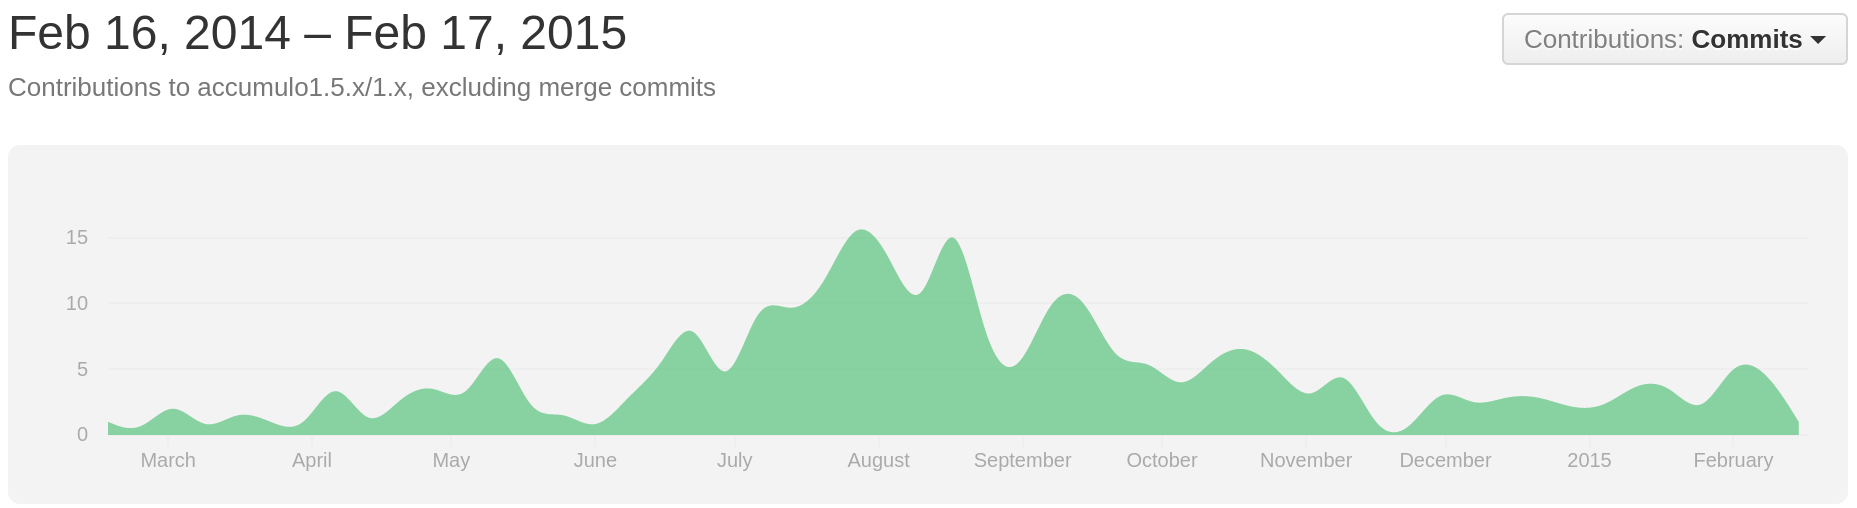
\includegraphics[width=\textwidth]{Abbildungen/geomesa_timeline_contributors.png}
\caption[Zeitleiste der contributor von GeoMesa]{Zeitleiste der contributor von GeoMesa vom 17.2.2015 nach \url{https://github.com/locationtech/geomesa/graphs/contributors}}
\label{fig:timeline_contr_geomesa}
\end{figure}
\begin{figure}[h!]
\centering
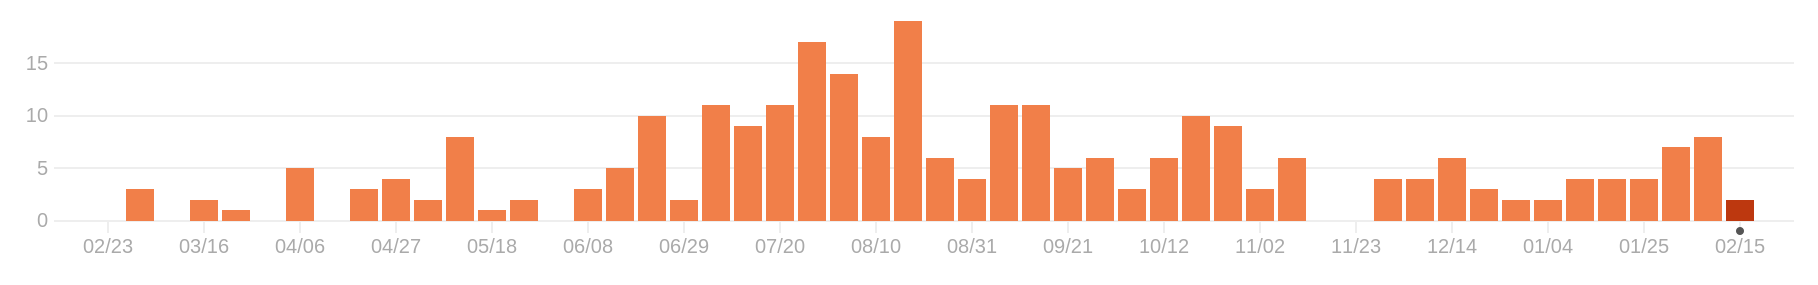
\includegraphics[width=\textwidth]{Abbildungen/geomesa_timeline_commits.png}
\caption[Zeitleiste der commits von GeoMesa]{Zeitleiste der commits von GeoMesa vom 17.2.2015 nach \url{https://github.com/locationtech/geomesa/graphs/commit-activity}}
\label{fig:timeline_commits_geomesa}
\end{figure}
Das GeoMesa Projekt auf GitHub hat nach Abbildung \ref{fig:timeline_contr_geomesa} eins bis vier Stammprogrammierer und ist im zweiten und dritten Quartal gegenüber mit der doppelten Anzahl an contributors gegenüber den anderen Quartalen fragmentiert.
Die drei contributors mit dem größten Anteil an Änderungen sind vorwiegend in Projekten von LocationTech aktiv was darauf schließen lässt, dass sie für das Unternehmen arbeiten.
Daraus folgt das zum wesentlichen Teil das Unternehmen LocationTech das Projekt wartet.
Die Anzahl der commits geht mit dem Verlauf der aktiven Programmierer einher.
Abbildung \ref{fig:timeline_commits_geomesa} zeigt die selbe Quartalsweise Verteilung wie Abbildung \ref{fig:timeline_contr_geomesa}.
Dabei ist der Unterschied zwei zu neun commits pro Woche.

LocationTech ist eine Arbeitsgruppe der non-for-profit Stiftung Eclipse.
In diesem Rahmen erhält diese Arbeitsgruppe 20 Mitglieder für Projektplanung und Projektumsetzung.
Weiterhin findet die Finanzierung im Rahmen von Mitgliedschaft an der Arbeitsgruppe statt.
Darin können Mitglieder je nach Beitrag Teile der Entscheidungsorgane der Arbeitsgruppe werden und Zugang zu Ergebnissen dieser erhalten. \cite{website:locationtech-about}
LocationTech ist mit GeoMesa mitten in der Entwicklung und hat keine permanenten aktive Unterstützer.
Dieser Stand spricht gegen eine Auswahl von GeoMesa zum produktiven Einsatz.

\section{Postgres-XL}

\subsection{Interoperabilität}
\begin{description}
\item[PostgreSQL - 7] PostgreSQL ist Bestandteil von Postgres-XL wobei die Datentypen vollständig verfügbar sind.
\item[\Gls{umn} - 5] Mit der Erweiterung Postgis direkt als Quelle für \Gls{umn} angebbar. \cite{website:umn-layer}
\end{description}
Die Wertung für Interoperabilität ist somit 12 mit einer Erfüllung von 100\%.

\subsection{Funktionsumfang}
\begin{description}
\item[Parallele Verarbeitung - 2] Verteilte Datenhaltung mit partitioning der Daten und verschränkte parallele Datenverarbeitung mit \Gls{mpp} möglich. \cite{website:postgresxl-overview}
\item[Geografische Datentypen - 14] Vollständige Datentypen aus Simple Feature Access sowie PostGIS raster. \cite{website:postgisdocu-opengis}
\item[Umrechnungsfunktionen - 10] Direkter Funktionsaufruf zur Umrechnung von und in beliebige EPSG Codes. \cite{website:postgis-updatesrid} %TODO: EPSG erklären
\item[Gruppierungsfunktionen - 10] SQL in PostgreSQL mit der Erweiterung PostGIS erlaubt beliebige Querys mit geografischen Daten. \cite{website:postgisdocu-opengis}
\item[Verschneidungsfunktionen - 3] Funktionsübersicht zeigt intersection, difference und symmetric difference. \cite{website:postgisdocu-functions}
\item[Overlayfunktionen - 2] Funktionsübersicht zeigt relation und intersects. \cite{website:postgisdocu-functions}
\item[Geostatistik - 2] Interpolation nur von Linie zu Punkt mit PostGIS möglich. Jedoch kann mit R oder C++ beliebige Geostatistik mit vorhandenen und eigenen Funktionen durchgeführt werden.
\item[Filterfunktionen - 10] In SQL mit mehreren Funktionen. \cite{website:postgisdocu-functions}
\item[Schemaversionierung - 0] Nicht eingebaut. Mit eigenen Skripten möglich.
\end{description}
Daraus ergibt sich ein Wert von 53, was 87\% des maximal zu erreichenden Wertes ist.

\subsection{Dokumentation}
\begin{description}
\item[Installation - 1] Knapp auf \cite{website:postgresxl-install} beschrieben.
\item[Zeitverhalten - 0] Keine Angaben.
\item[Funktionsumfang - 2] Es existiert eine Übersicht zur Verwaltung eines Postgres-XL Clusters. Dazu ist die allgemeine Dokumentation zu PostgreSQL und PostGIS verfügbar. \cite{website:postgresxl-manual}
\item[Interoperabilität - 2] Verweis auf Dokumentation von PostgreSQL und PostGIS sowie API auf \cite{website:postgresxl-api}.
\item[Best Practise - 1] Einige Hinweise auf \cite{website:postgresxl-manual} vorhanden.
\item[Anpassbarkeit - 3] \cite{website:postgresxl-extend} dokumentiert Erweiterung mit SQL, tcl, Perl und Python.
\end{description}
Das Qualitätskriterium Dokumentation wird für Postgres-XL mit dem Wert 9, bzw. der Erfüllung von 69\%,  belegt.

\subsection{Modifizierbarkeit}
\begin{description}
\item[Verwendung eigener Datentypen - 1] Mit PostgreSQL eigene Datentypen erstellbar.
\item[Erstellung eigener Schnittstellen - 1] Für eigene Programme mit JDBC oder ODBC Daten verwendbar.
\item[Erstellung eigener Funktionen - 1] Ebenso mit SQL möglich.
\item[Verwendung der Programmiersprachen Scala oder R - 1] R kann direkt in SQL Funktionen eingebettet werden. Scala ist mit JDBC verwendbar.
\item[Anlegen eigener Berechnungsvorgängen zur späteren Abarbeitung - 1] Hier sind Trigger und selbstständige Programme mit JDBC Nutzung zu nennen.
\end{description}
Hier ist die Wertung 5 von 5 Punkten und damit 100\%.

\subsection{Zusammenfassung}
\begin{table}[h!]
\centering
\small
\begin{tabular}{l|p{1.8cm}|c|p{3.1cm}|p{1.8cm}}
\textbf{Metrik} & \textbf{erreichter Wert} & \textbf{Erfüllung in \%} & \textbf{Kommentar} & \textbf{gewichteter Teilnutzen} \\ \hline
Interoperabilität & 12 & 100 & analog Ist-Stand & 30 \\ \hline
Funktionsumfang & 53 & 87 & Geostatistik und Versionierung nicht vorhanden & 17 \\ \hline
Dokumentation & 9 & 69 & Dokumentation zu PostGIS sehr gut, zu Postgres-XL grob & 24 \\ \hline
Modifizierbarkeit & 5 & 100 & Bereits in SQL gegeben. & 15 \\
\end{tabular}
\caption{Nutzwertanalyse Postgres-XL}
\label{table:nutzwertanalyse-postgresxl}
\end{table}
Aus Tabelle \ref{table:nutzwertanalyse-postgresxl} ergibt sich ein Nutzwert von 86.\\
Dazu sind ebenso nichttechnische Faktoren zu berücksichtigen.\\
\url{https://github.com/snaga/postgres-xl} zählt am 17.2.2015 35.266 commits, 23 contributors und drei branches.
\begin{figure}[h!]
\centering
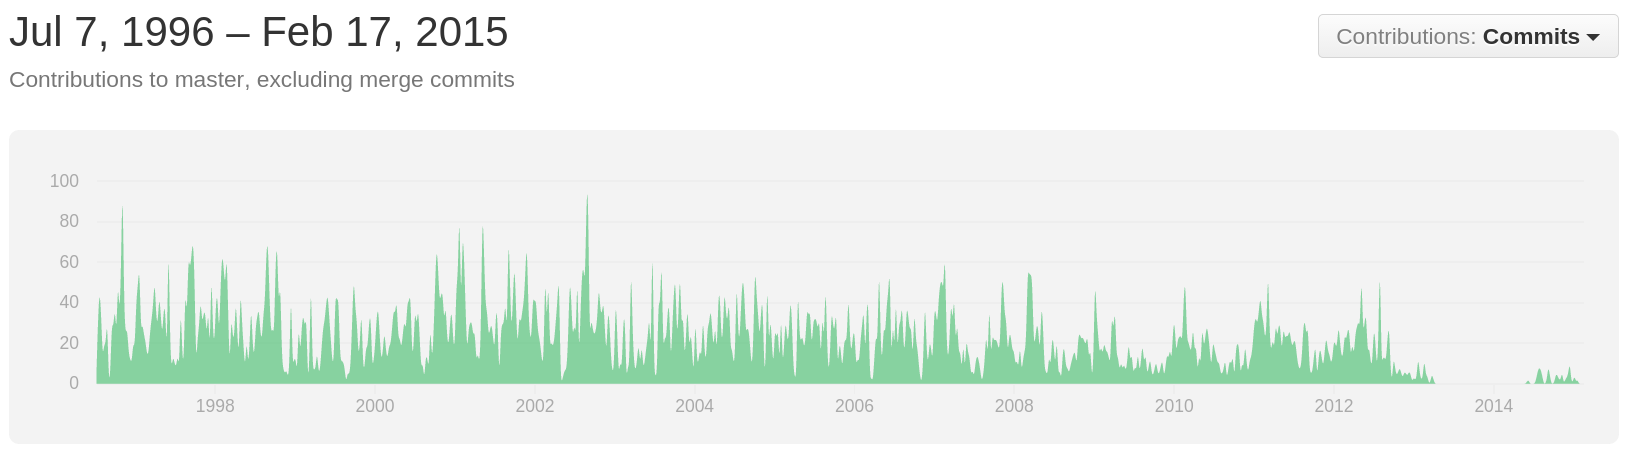
\includegraphics[width=\textwidth]{Abbildungen/postgresxl_timeline_contributors.png}
\caption[Zeitleiste der contributor von Postgres-XL]{Zeitleiste der contributor von Postgres-XL vom 17.2.2015 nach \url{https://github.com/snaga/postgres-xl/graphs/contributors}}
\label{fig:timeline_contr_postgresxl}
\end{figure}
\begin{figure}[h!]
\centering
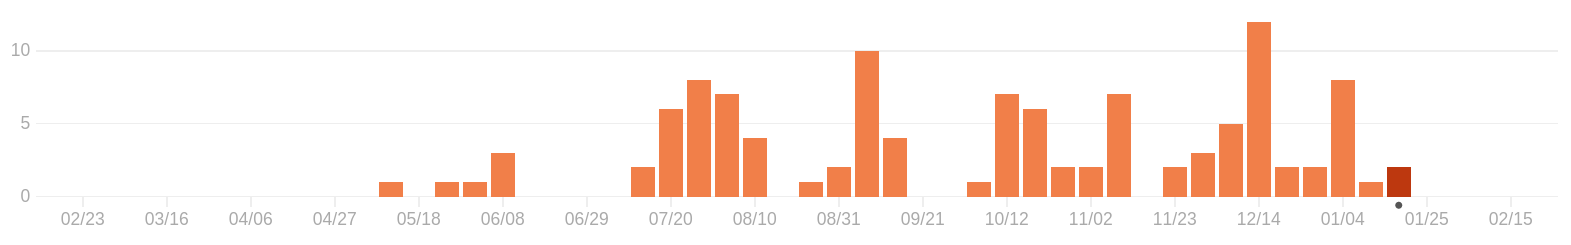
\includegraphics[width=\textwidth]{Abbildungen/postgresxl_timeline_commits.png}
\caption[Zeitleiste der commits von Postgres-XL]{Zeitleiste der commits von Postgres-XL vom 17.2.2015 nach \url{https://github.com/snaga/postgres-xl/graphs/commit-activity}}
\label{fig:timeline_commits_postgresxl}
\end{figure}
Abbildung \ref{fig:timeline_contr_postgresxl} zeigt einerseits, dass dieses Projekt seit 1998 besteht, andererseits das die Zahl der aktiven contributors im Gegensatz der Jahre 1998 bis 2012 zu 2014/2015 in etwa ein viertel beträgt.
Diese starke abrupte Abnahme der aktiven Programmierer deutet eine Veränderung im Projekt oder den Projektverantwortlichen an.
Die commits des vergangenen Jahres sind in Abbildung \ref{fig:timeline_commits_postgresxl} dargestellt.
Danach wurden im ersten Halbjahr 2014 nur insgesamt 6 commits und im zweiten Halbjahr 2014 etwa täglich ein commit durchgeführt.

Das Unternehmen TransLattice übernahm im Mai 2014 das Unternehmen StormDB.
Die Übernahme schloss das Projekt Postgres bzw. Postgres-XC ein. (siehe \cite{website:translattice-stormdb})
Dieses wurde darauf in Postgres-XL umbenannt und erweitert.
Diese Änderung rief die Verringerung der contributors seit Anfang 2014 hervor.
TransLattice verwaltet seitdem das Projekt und stellt technischen sowie theoretischen Support.
Postgres-XL ist durch die langjährige Entwicklung empfehlenswert für den produktiven Einsatz.
Jedoch ist die Aktivität der TransLattice Entwickler zu beobachten, da die Gefahr besteht das dieses Projekt vom Unternehmen nicht mehr gefördert wird und somit Fehler und Verbesserungen nicht eingepflegt werden und neue PostgreSQL Versionen nicht unterstützt werden.


\section{Rasdaman}

\subsection{Interoperabilität}
\begin{description}
\item[PostgreSQL - 7] PostgreSQL wird nach \cite{website:rasdaman-features} unterstützt.
\item[\Gls{umn} - 5] Als Datenquelle ist Rasdaman als \Gls{wcs_glos} und \Gls{wps_glos} Dienst in \Gls{umn} verwendbar.
\end{description}
Die Wertung für Interoperabilität ist somit 12 mit einer Erfüllung von 100\%.

\subsection{Funktionsumfang}
\begin{description}
\item[Parallele Verarbeitung - 1] Parallele Server Instanzen verwendbar. In der kostenlosen Version keine Query Optimierung für mehrere Kerne und Instanzen vorhanden. \cite{website:rasdaman-features}
\item[Geografische Datentypen - 4] Raster und Punkte sind für die räumliche Datenverarbeitung vorhanden. Dazu sind Arrays mit beliebig vielen Dimensionen verwendbar. \cite{website:rasdaman-introduction}
\item[Umrechnungsfunktionen - 0] Nur mit externer Bibliothek \Gls{gdal} für zwei-dimensionale Arrays möglich. \cite{website:rasdaman-gdal}
\item[Gruppierungsfunktionen - 0] Laut Dokumentation der Funktionen keine Gruppierung möglich. \cite{website:rasdaman-querymanual}
\item[Verschneidungsfunktionen - 1] Dagegen sind einfache Array Operationen vorhanden.
\item[Overlayfunktionen - 1] Ditto.
\item[Geostatistik - 0] Keine eingebaute Funktionalität.
\item[Filterfunktionen - 5] Operationen für Array-Verarbeitung vorhanden.
\item[Schemaversionierung - 0] Keine eingebaute Funktionalität.
\end{description}
Daraus ergibt sich ein Wert von 12, was 20\% des maximal zu erreichenden Wertes ist.

\subsection{Dokumentation}
\begin{description}
\item[Installation - 1] \cite{website:rasdaman-dokumentation} ist eigenes Installationsdokument.
\item[Zeitverhalten - 0] Keine Dokumentation vorhanden.
\item[Funktionsumfang - 2] Ist grob unter \cite{website:rasdaman-features} beschrieben und detailiert in \cite{website:rasdaman-querymanual} aufgeführt.
\item[Interoperabilität - 3] Interoperabilität mit PostgreSQL und API unter \cite{website:rasdaman-querymanual} verfügbar.
\item[Best Practise - 1] Einzig Hinweise verfügbar. \cite{website:rasdaman-installationguide}
\item[Anpassbarkeit - 1] Kein eigenständiges Dokument vorhanden, erschließt sich aber aus genannten Quellen.
\end{description}
Das Qualitätskriterium Dokumentation wird für Postgres-XL mit dem Wert 8, bzw. der Erfüllung von 62\%, belegt.

\subsection{Modifizierbarkeit}
\begin{description}
\item[Verwendung eigener Datentypen - 0] Keine eigenen Datentypen erstellbar. Einzig die Verwendung von selbst definierten Arrays ist verfügbar.
\item[Erstellung eigener Schnittstellen - 1] Über \Gls{jdbc}/\Gls{odbc} in Java und C++ möglich.
\item[Erstellung eigener Funktionen - 1] In der Abfragesprache rasql nicht möglich, dagegen mit API.
\item[Verwendung der Programmiersprachen Scala oder R - 1] Scala mit API verwendbar.
\item[Anlegen eigener Berechnungsvorgängen zur späteren Abarbeitung - 0] Nicht vorgesehen.
\end{description}
Hier ist die Wertung 3 von 5 Punkten und damit 60\%.

\subsection{Zusammenfassung}
\begin{table}[h!]
\centering
\small
\begin{tabular}{l|p{1.8cm}|c|p{3.1cm}|p{1.8cm}}
\textbf{Metrik} & \textbf{erreichter Wert} & \textbf{Erfüllung in \%} & \textbf{Kommentar} & \textbf{gewichteter Teilnutzen} \\ \hline
Interoperabilität & 12 & 100 & UMN MapServer Schnittstelle nur indirekt vorhanden & 30 \\ \hline
Funktionsumfang & 12 & 20 & Umfangreiche Rasterverarbeitung möglich. Kostenlose Version enthält keine Optimierungen. & 4 \\ \hline
Dokumentation & 8 & 62 & Mehrere Dokumente vorhanden & 22 \\ \hline
Modifizierbarkeit & 3 & 60 & einfache Java und C++ API & 9 \\
\end{tabular}
\caption{Nutzwertanalyse Rasdaman}
\label{table:nutzwertanalyse-rasdaman}
\end{table}
Aus Tabelle \ref{table:nutzwertanalyse-rasdaman} ergibt sich ein Nutzwert von 65.



